% This LaTeX document needs to be compiled with XeLaTeX.
\documentclass[10pt]{article}
\usepackage[utf8]{inputenc}
\usepackage{graphicx}
\usepackage[export]{adjustbox}
\graphicspath{ {./images/} }
\usepackage{amsmath}
\usepackage{amsfonts}
\usepackage{amssymb}
\usepackage[version=4]{mhchem}
\usepackage{stmaryrd}
\usepackage[fallback]{xeCJK}
\usepackage{polyglossia}
\usepackage{fontspec}
\setCJKmainfont{Noto Serif CJK SC}

\setmainlanguage{english}
\setmainfont{CMU Serif}

\title{【题目描述】 }

\author{}
\date{}


\begin{document}
\maketitle
顿顿想要建立一个简单的教务管理数据库, 用于存储学生的考试成绩并支持一些基本的查询操作。

\section*{数据格式}
该数据库包含以下五张数据表:

Student(sid, dept, age)

学生信息表: sid 为主键, 表示学生 ID; dept 表示学生所在院系名称; age 表示学生的年龄。

Course(cid, name)

课程信息表: cid 为主键, 表示课程 ID; name 表示课程名称。

Teacher(tid, dept, age)

教师信息表: tid 为主键, 表示教师 ID; dept 表示教师所在院系名称; age 表示教师的年龄。

Grade(sid, cid, score)

成绩信息表: sid 和 cid 分别米自 Student 表和 Course 表的主键(即每条记录中的 sid 和 cid 一定存在于相应的表中, 下同), 二者一起作为该表的主键; score 表示该学生这门课程的成绩。

Teach(cid, tid)

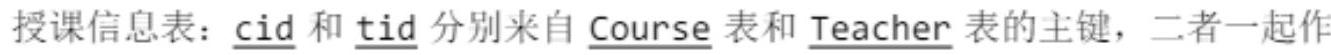
\includegraphics[max width=\textwidth, center]{2024_05_27_59dabe7159470efca570g-1}\\
为该表的主键; 需要注意的是, 一门课程可以有多个老师授课。

注: 主键 (Primary Key) 可以唯一标识表中的每条记录, 换言之在一张表中所有记录的主键互不相同。

在上述表中, age 和 score 是 $[0,100]$ 的整数, 其余都是长度小于等于 10 的非空字符串。其中三个主铤 sid $\underline{\text { cid }}$ 和 tid 由数字 $\underline{0 \ldots 9}$ 组成, 而 name 和 dept 则由大小写字丹组成。

\section*{查询语句}
该数据库支持使用一种简单的 SELECT 语句进行查询, 文法定义如下所述。最终所有的查询语句都可以由 QUERY 符号推导而来。

在所有定义中, $::=$ 衣示其左侧的符号可以推导为右侧的符号串, 其中带单引号的符号衣示此符号为周定的字符串, 不带引号的则衣示符号还需要进行进一步推导。[衣示文法中的可选内容。如果一个符号存在多种推导方式 A ::= B 和 A : := C, 则可以简"与为 $A::=B \mid C$ 。

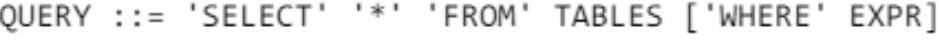
\includegraphics[max width=\textwidth, center]{2024_05_27_59dabe7159470efca570g-2}\\
QUERY ::= 'SELECT' COLUMNS 'FROM' TABLES [<WHERE' EXPR]

\begin{verbatim}

从指定的表(TABLES) 中查询满足䇜选条件(EXPR)的记录, 并按照指定的列 (COLUMNS) 输出。如果没有给出笠选条件, 则返回所有的记录。

TABLES : $:=$ TABLE_NAME | TABLE_NAME ',' TABLE_NAME

TABLE_NAME ::= 'Student' | 'Grade' | 'Course' | 'Teach' | 'Teacher'

TABLES 可以包含多张表, 此时新衣中的列是这些衣中列的笛卡尔积, 一个例子如下所示。

![](https://cdn.mathpix.com/cropped/2024_05_27_59dabe7159470efca570g-2.jpg?height=517&width=997&top_left_y=1272&top_left_x=381)

本题中约定 TABLES 仅会包含一张或两张不同的表。

COLUMNS : $:=$ COLUMN | COLUMNS ', COLUMN

COLUMN : $:=[$ TABLE_NAME '.

COLUMN_NAME ::= 'sid' | 'cid' | 'tid' | 'age' | 'score' | 'dept' | 'name'

COLUMNS 也是递归定义, 即由远号分隔的至少一个 COLUMN 组成。在无歧义时(即 TABLES 中只有唯一的表含有该列), COLUMN 中的 TABLE_NAME 是可选的。 SELECT age

FROM Student, Teacher 是一种典型的歧义句式, 因为无法确定其中想要选取的 age 是学生还是教师的年龄。

虽然在文法上一个 COLUMN 可以由任意 TABLE_NAME 和 COLUMN_NAME 组合而成,但在实际处理时, 这两者需要符合上而定义的表结构。比如 Course.sid 就是一种错误的写法, 因为 Course 表中并没有 sid 这一列。

EXPR ::= COND | EXPR 'AND' COND

COND ::= COLUMN CMP CONSTANT | COLUMN '=' COLUMN

CMP ::= '>' | '=' | '<'

其中:
- EXPR 是一个合取布尔表达式, 由若下个比较条件(COND)用 AND 连接而成, 表示篮选条件 (即满足该条件的记录才会被输出)。
- CONSTANT 没有文法定义, 它表示一个常量, 且其类型和数据范困与相比较的 COLUMN 一致; 如果是字符串类型, 还需用双引号括起 (例如 "Sam")。

这里我们额外规定:
- 列与常量进行比较时 (COLUMN CMP CONSTANT), 整数类型 (age、score) 可以进行大于、小于和等于三种判断, 字符串类型只能做等于灲断;
- 两列进行比较时 (COLUMN = COLUMN), 它们需米自不同的表且二者的列名 (COLUMN_NAME) 必须相同;
- 在一个 EXPR 中, COLUMN CMP CONSTANT 类型的 COND 个数不限, 但 COLUMN = COLUMN 最多只能出现一次。

查询语句大小写敏感, 全部的保留字包括:

SELECT, *, FROM, WHERE, AND, Student, Course, Teacher, Grade, Teach sid, cid, tid, dept, name, age, score

![](https://cdn.mathpix.com/cropped/2024_05_27_59dabe7159470efca570g-3.jpg?height=57&width=688&top_left_y=1728&top_left_x=387)

双引号 (") 应视作字符串常量的一部分而非保留字或分隔符。

每个保留字和常量 (CONSTANT) 可视作查询语句中的一个基本单位, 在格式上我们约定:
- 每条查询语句占一行;
- 基本单位不可分割;
- 为避免歧义, 两个基本单位之间应至少有一个分隔符, 并且允许存在任意多的空格;
- 一行总长度不超过 100 个字符。

\section*{结果输出}

对每条查询输出一张表, 列由 COLUMNS 指定, 每行为一条满足师选条件 (EXPR)的记录 (不同的列间用一个空格分隔)。这里只需要输出所有满足条件的记录, 不需罗打印表头; 查询炶果为空则不输出; 字符串类型无需输出双引号。若想输出所有的列,可以用 $\underset{*}{*}$ 代替 COLUMNS; 若 TABLES 中只有一张表, 此时应输出该表的全部列; 如果有第二张表,应输出第一张表的全部列与二张表的全部列的笛卡尔积:表内部的列按照上文定义时给出的顺序排序。

如果 TABLES 仅含一张表, 则按该表的顺序依次输出符合条件的记录。若 TABLES 包含两张表(形如 $\underline{A, B}$ ), 则先考虑 $A$ 的顺序, 再考虑 $B$ 的顺序(参考前文中两张表做笛卡尔积的例子)。

\section*{【输入格式】}

从标准输入读入数据。

首先依次输入五张表 Student、Course、Teacher、Grade 和 Teach 的数据。

对于第 $i$ 张表, 第一行输入一个正整数 $N_{i}$, 表示该表中记录的个数(亦即行数)。接下来 $N_{i}$ 行, 每行输入一条记录, 其中不同列之间用一个空格分隔且字符出字段不会用双引号括起。

然后输入一个正整数 $M$, 表示需要处理的查询语句个数。最后 $M$ 行每行输入一条查询语句, 保证每条查询语句均符合上述所有要求。

\section*{【输出格式】}

输出到标准输出。

按要求输出每条查询语句的炶果。

\section*{【样例 1 输入】}

3

2019001 law 19

2019002 info 20

2019003 info 19

2

20190001 math

20190002 English

2

2019101 info 49

2019102 info 38

\section*{4}

SELECT * FROM Student

SELECT Student . dept FROM Student

SELECT Student.sid,Grade.sid,dept, score FROM Student,Grade

SELECT * FROM Student, Grade WHERE Grade .sid=Student. sid

\section*{【样例 1 输出】}

\end{verbatim}

2019001 law 19\\
2019002 info 20\\
2019003 info 19\\
law\\
info\\
info\\
2019001 2019002 law 100\\
2019001 2019003 law 0\\
2019002 2019002 info 100\\
2019002 2019003 info 0\\
2019003 2019002 info 100\\
2019003 2019003 info 0\\
2019002 info 20 2019002 20190001 100\\
2019003 info 19 2019003 20190002 0

\begin{verbatim}

\section*{【样例 1 解释】}

第 1-3 行、4-6 行、7-12 行和 13-14 行依次对应四条查询的炶果。

每条查询最多涉及两张表,每个 expr 中最多一个 COLUMN = COLUMN 类型的 COND,且 $N i \leqslant 10000 、 M \leqslant 10$ 。此外,所有测试数据保证每条查询的结果均不超过 10000 行。
\end{verbatim}


\end{document}